%
%
\documentclass[12pt]{scrartcl}

% own geometry
\usepackage[a4paper, left=3cm, right=3cm]{geometry}

\usepackage[ngerman]{babel} 
\usepackage[utf8]{inputenc} 
\usepackage[T1]{fontenc}
\usepackage{graphicx}
\usepackage{color}
\usepackage{xcolor}
\usepackage{jurabib}
\usepackage{hyperref}
\usepackage{here} % picture positioning
\usepackage{pdfpages}

\usepackage{latexsym} 
\newcommand*{\thecheckbox}{\hss$\Box$} 
\newenvironment*{checklist} 
{\list{}{% 
\renewcommand*{\makelabel}[1]{\thecheckbox}}} 
{\endlist} 

\renewcommand*{\jbauthorfont}{\textsc}
\renewcommand*{\bibfnfont}{\normalfont}
\renewcommand*{\biblnfont}{\textsc}
%\renewcommand*{\samepageibidemname}{Ebd.}
\renewcommand*{\bibbtsep}{In: }
\renewcommand*{\bibjtsep}{In: }
\renewcommand*{\bibpldelim}{(}
\renewcommand*{\biburlprefix}{}
\renewcommand*{\biburlsuffix}{}

\makeatletter
\renewcommand*{\jbshorttitlefont}{%
\ifthenelse{%
\equal{\jb@@type}{article}%
\or
\equal{\jb@@type}{periodical}%
\or
\equal{\jb@@type}{incollection}%
}{%
\upshape%
}{%
\textit%
}%
}
\makeatother

\renewcommand*{\bibprdelim}{)}
\renewcommand*{\ajtsep}{}
\renewcommand*{\bpubaddr} { :}
\renewcommand*{\jbbtasep} { ; }
\renewcommand*{\jbbfsasep} { ; }
\renewcommand*{\jbbstasep} { ; }
\renewcommand*{\bibbtasep} { ; }
\renewcommand*{\bibbfsasep} { ; }
\renewcommand*{\bibbstasep} { ; } %between second and third author sep
\renewcommand*{\jbbtesep} { ; } %between two editors sep
\renewcommand*{\jbbfsesep} { ; } %between first and second editor sep
\renewcommand*{\jbbstesep} { ; } %between second and third editor sep
\renewcommand*{\bibbtesep} { ; } %between two editors sep
\renewcommand*{\bibbfsesep} { ; } %between first and second editor sep
\renewcommand*{\bibbstesep} { ; } %between second and third editor sep
\AddTo\bibsgerman{\def\editorsname{(Hrsg.)}}
\AddTo\bibsgerman{\def\editorname{(Hrsg.)}}
%\jurabibsetup{super, citefull=first,ibidem}
%\jurabibsetup{ibidem}
%\jurabibsetup{authorformat=citationreversed}
%\jurabibsetup{authorformat=reducedifibidem}
\jurabibsetup{biblikecite}
%\jurabibsetup{bibformat=ibidem}
%\jurabibsetup{pages=always}
\jbfirstcitepageranges
\AddTo\bibsgerman{\def\herename{hier}}
\jbuseidemhrule

\jurabibsetup{
  authorformat={smallcaps,year,and,citationreversed},
  titleformat={colonsep,all,italic},
  commabeforerest,
  see,
  dotafter=bibentry,
  ibidem=strict,
  biblikecite
}

\renewcommand*{\bibbtasep}{ und } %
\renewcommand*{\bibbfsasep}{, }   %
\renewcommand*{\bibbstasep}{ und }
\renewcommand*{\jbtitlefont}{}
\renewcommand*{\bibtfont}{}
\renewcommand*{\bibbtfont}{}
\renewcommand*{\bibjtfont}{}
\renewcommand*{\bibapifont}{}
\renewcommand*{\jbshorttitlefont}{}



	%
	% CITATIONS
	%
\newcommand{\book}[2]{\footnote{\cite[Vgl.][#2]{#1}}}
\newcommand{\bookwf}[2]{\cite[Vgl.][#2]{#1}}
\newcommand{\bookdir}[2]{\footnote{\cite[][#2]{#1}}}
\newcommand{\inetwf}[1]{\cite[Vgl.][\citefield{url}{#1}]{#1}}
\newcommand{\inetwfdir}[1]{\cite[][\citefield{url}{#1}]{#1}}
\newcommand{\inet}[1]{\footnote{\inetwf{#1}}}
\newcommand{\inetdir}[1]{\footnote{\cite[][\citefield{url}{#1}]{#1}}}
\newcommand{\innerref}[1]{\footnote{Vgl. auch Kapitel \ref{#1} dieser Arbeit, S. \pageref{#1}}}
\newcommand{\vgl}[2]{\cite[Vgl.][#2]{#1}}
\newcommand{\citeauthoryear}[1]{\citeauthor{#1} (\citeyear{#1})}
\bibliographystyle{jurabib}

% setup of source code listings
\usepackage{listings}
%\usepackage{courier}
\usepackage{caption}

\DeclareCaptionFont{white}{\color{white}}
\DeclareCaptionFormat{listing}{\colorbox{gray}{\parbox{\textwidth}{#1#2#3}}}
\captionsetup[lstlisting]{format=listing,labelfont=white,textfont=white}

% layout the box
%\DeclareCaptionFormat{listing}{\colorbox[rgb]{0.43, 0.35, 0.35 {\parbox{\textwidth}{\hspace{15pt}#1#2#3}}}

% Headings
\usepackage{fancyhdr}
\renewcommand{\footrulewidth}{1pt}
%\fancyhead[R]{\colorbox{blue!20}{ Oliver Erxleben}}
\fancyfoot[C]{}
\fancyfoot[R]{\thepage}

% Document begins now
\begin{document}

\author{
	Oliver Erxleben \small(\href{mailto:oliver.erxleben@hs-osnabrueck.de}{oliver.erxleben@hs-osnabrueck.de})\\ \\%
	%
	Hochschule Osnabr"uck \\%
	Ingenieurswissenschaften und Informatik \\%
	Informatik - Mobile und Verteilte Anwendungen }

\title{
\includegraphics[scale=0.75,keepaspectratio]{img/hs_os.png}\linebreak \linebreak Probleme im Projektmanagement und Führungstipps}

\maketitle
\thispagestyle{empty}
\pagebreak
\thispagestyle{empty}
\tableofcontents
\listoffigures
\thispagestyle{empty}
\pagebreak
\thispagestyle{empty}
\begin{abstract}
\textbf{Zusammenfassung}\\
Die vorliegende Arbeit wurde mit LaTex verfasst und ist eine Arbeit von Oliver Erxleben für das Modul \textit{Projektmanagement und Führungstheorien} aus dem Master-Studiengang \textit{Informatik - Verteilte und Mobile Anwendungen} der \textit{Hochschule Osnabrück / University of Applied Sciences}.\\
\\
Das Thema der Arbeit lautet \textbf{Probleme im Projektmanagement und Führungstipps}. Es wird auf typische Problemstellen eines Projekts eingegangen, mit der das Projektmanagement konfrontiert wird.\\
Die Arbeit ist in mehrere Abschnitte aufgeteilt. In der Einleitung wird nach der Motivation für Probleme im Projektmanagement auf Eckdaten und Begriffsdefinitionen eingegangen.\\
\\
Der Abschnitt 2 befasst sich mit Studien um den Trend des Projektmanagements und der Projektmanagementkultur, sowie einer Studie der GPM, die versucht Erfolgsfaktoren für Projekte zu ermitteln.\\
\\
Die darauffolgenden Abschnitte schildern Probleme aus den aus Abschnitt zwei ermittelten Erfolgsfaktoren für Projekte.\\
\\
Im letzten Abschnitt werden die Erkenntnisse resümiert und ein Ausblick gegeben, wie Problemen in Zukunft vorgebeugt werden können.\\
\\
Es sei erwähnt dass die Arbeit auf IT-Projekte abzielt. Besonders werden IT-Projekte, bzw. Projekte in der Software-Entwicklung betrachtet. Projektmanagement aus anderen Branchen, wie Bauingenieurswesen oder Projektmanagement im Gesundheitswesen, wird in dieser Arbeit nicht betrachtet. 
\end{abstract}

\pagebreak
% set new page style

\pagestyle{fancy}
\setcounter{page}{1} 

\section{Einleitung}

Projekte scheitern! Projekte scheitern in der IT häufiger als sie Erfolg haben. Und das obgleich die Disziplin des \textit{''Projektmanagaments''} keine neue Erfindung ist und diese sich ständig weiter entwickelt und verstärkte Aufmerksamkeit in Unternehmen erfährt. So ist in den letzten Jahren zu verzeichnen, dass Projektportfolios und Projektauswahl mit der Unternehmens- und Geschäftsfeldstrategie abgestimmt werden. Fakt ist das Strategien, Produkte, Dienstleistungen oder Innovationen durch Projekte realisiert werden. Dies wird in Unternehmen immer mehr thematisiert.\\
Diese Tendenz ist zwar positiv, aber aufgrund der harten Fakten in Studien trotz allem scheinbar nicht genug. Studien belegen das 46 \%\footnote{''Chaos-Report'' der Standish Group 2006} der IT-Projekte in Deutschland Wünsche und Anforderungen von Auftraggebern nur teilweise oder gar nicht erfüllt haben. Hinzukommt das 20 \% von IT-Projekten abgebrochen und nur 16 \% der IT-Projekte können als \textit{erfolgreich} eingestuft werden können. Warum also scheitern so viele Projekte in der IT und welche Probleme und Problemsituationen gibt es in einem Projekt? Sind die Fachkompetenzen zu gering? Sind die Ziele eines Projekts zu hoch gegriffen? Ist die Führungsebene eines Unternehmens schuld? Oder arbeiten alle einfach nur zu wenig?\\
Ähnliche Ergebnisse zum Erfolg bzw. Misserfolg eines Projekts liefert auch eine Studie der GPM\footnote{deutsche Gesellschaft für Projektmanagement e.V.}, in der mögliche Probleme in IT-Projekten und Ursachen für das Scheitern von Projekten erforscht werden (Details siehe Abschnitt \ref{studies_gpm}).\\ 
Jedes Projekt, egal ob erfolgreich oder nicht, hat oder hatte Probleme zu verzeichnen. Seien es nun Probleme, wie z.B. Interessenskonflikte zwischen Projektbeteiligten und -mitarbeitern, sich ändernde Anforderungen oder die Schwierigkeit das Projekt im Projektverlauf kontinuierlich zu steuern und zum Erfolg zu führen.\\
Es ist die Kunst der Führung und des Projektmanagements, sowie der Führungsebene sich bildende oder aftretende Probleme  und kritische Phasen innerhalb eines Projekts frühzeitig zu erkennen, vorzubeugen oder schnell zu lösen. Dies bedarf allerdings Probleme eines Projekts und damit Probleme des Projektmanagements zu erkennen und durch geeignete Operationen in der Führung diese Probleme zu lösen.

\pagebreak
\subsection{Aufbau und Ablauf der Arbeit}
Die vorliegende Arbeit gliedert sich in sechs Abschnitte: Einleitung, Projekte Scheitern, Kommunikationsprobleme, Projektziele, Teambesetzung und Projektleiter, sowie dem Fazit.\\
\\
Im einleitenden Teil wird in das Thema der Arbeit eingeführt und wichtige Begriffe für die restliche Arbeit definiert und abgegrenzt.  
\\ \\
Der darauffolgende Teil der Arbeit beschäftigt sich mit der aktuellen Lage in der Projektmanagementkultur und wertet Studien aus, die zeigen welche Faktoren maßsgeblich für erfolgreiche Projekte sind und leiten die wichtigen Erfolgsfaktoren für Projekt ab, die in der vorliegenden Arbeit in den weiteren Abschnitten erläutert werden. 
\\ \\
Im Teil Fazit werden Erkenntnisse aus dem Hauptteil zusammengefast und bewertet.

\subsection{Begriffsdefinitionen}

Im Folgenden werden zentrale Begriffe für die Arbeit definiert, da es im World Wide Web und in diverser Fachliteratur und der DIN unterschiedliche Definitionen existieren. Missverständnisse sollen somit vermieden werden.

\subsubsection{Projekt}
Ein Projekt verfolgt immer ein Ziel, also eine bestimmte \textit{Zielvorgabe}, wie zum Beispiel die Umsetzung einer Auftragsarbeit. \\
\\
Ein Projekt wird nach Aussage der DIN-Begriffsnorm 69 901 allgemein defniniert durch \texttt{''ein Vorhaben, das im Wesentlichen durch die Einmaligkeit der Bedingung in ihrer Gesamtheit gekennzeichnet ist, wie z.B. 
\begin{itemize}
    \item{Zielvorgabe}
    \item{zeitliche, finanzielle, personelle und andere Begrenzungen}
    \item{Abgrenzung gegenüber anderen Vorhaben}
    \item{projektspezifische Organisation}
\end{itemize}''} gekennzeichnet. Im weiteren Vergleich mit \cite{proj_zum_erfolg_fuehren} (Kapitel 2, Seite 19 ff.) werden die in der DIN-Begriffsnorm eingetragenen Merkmale noch um die Beteiligung von Menschen, Arbeitsgruppen und Institutionen erwitert und die Existenz eines \textit{Ein-Personen-Projekts} ausgeschlossen. Mit beiden Ergänzungen und der DIN-Definition wird in den nachfolgenden Kapiteln ein Projekt verstanden. 

\subsubsection{Phasen, Meilensteine und Aktivitäten}

Unter \texttt{Projektphasen} werden Ereignisse in einem Phasenmodell\footnote{auch bez. als Phasenmodell, Vorgehensmodell, Prozessmodell} verstanden, die zeitleich aufeinander folgen. So kann das Testen einer Software beispielsweise nicht vor dessen Planungsphase stattfinden. Das Phasenmodell dient als Hilfsmittel im Projektmanagement. \\
\\
Ein \texttt{Meilenstein} ist im Vergleich zur Projektphase (nach DIN 69 900) \texttt{ein Ereignis besonderer Bedeutung}. Meist erhält ein Meilenstein einen geplanten Termin und Inhalte, die zu diesem Termin umgesetzt sein müssen. \\
\\
Zusätzlich zu Phasen und Meilensteine können auch \texttt{Aktivitäten} definiert werden. Sie beschreiben \textit{was} in den verschiedenen Projektabschnitten bearbeitet werden muss, um ein Teilergebnis erzielen zu können.  

\subsubsection{Projektmanagement}
Die DIN definiert Projektmanagement als \texttt{die Gesamtheit von Führungsaufgaben,\\ -organistion, -techniken und -mitteln für die Abwicklung eines Projekts}.\\
\\
Von der Disziplin \texttt{Projektmanagement} kann, wenn auch schon immer Vorhaben durchgeführt wurden, seit den 1950ern geredet werden. Geprägt wurde das Projektmanagement stark vom Militär und der Luft- und Weltraumindustrie der USA. Dort waren starke Termin- und Kostenüberschreitungen fatal für die Auftraggeber. Gerade die Luft- und Raumfahrtindustrie trug maßgeblich zu den anfänglichen Techniken im Projektmanagement bei\footnote{Vgl. \cite{proj_zum_erfolg_fuehren}, Die Entwicklung der Disziplin Projektmanagement, Seite 23 f.}. 
\\
Es kann aber auch als \textit{Führungskonzept} verstanden werden, bei dem die Aufgaben und Methoden des Projektmanagements mit die strategischen Ziele und der Entwicklung des Unternehmens verknüpft werden müssen (Vgl. \cite{scriptPM}, Seite 7). 

\subsubsection{Projektleitung}
Als Projektleitung wird die omni-verantwortliche Person für ein Projekt bezeichnet (Vgl. \cite{proj_zum_erfolg_fuehren}, Kap. 6 Seite 70 f., bezeichnet den Projektleiter als \texttt{Unternehmer auf Zeit im Unternehmen}). \\
\\
Der Projektleiter hat die Verantwortung über den Erfolg oder Misserfolg seines Projekts. Es ist \textit{sein} Projekt. Er ist verantwortlich für die Realisierung der definierten Projektziele, Termineinhaltung, Kosten- und Qualitätsgarantie und der Koordination der Projektbeteiligten. 

\subsubsection{Projektbeteiligte}
\label{proj_beteiligte}
% TODO: weitere Projektbeteiligte + Beschreibung
Neben dem Projektmanagement und der Projektleitung sind weitere Personen und Gruppen von Personen an einem Projekt beteiligt. Nach dem Skript, \cite{scriptPM}, Kap. 1.6. Personen und Beteiligte im Projektmanagement, Seite 6 f., können Projektbeteiligte in drei Personengruppen unterschieden werden: Kunden, Stakeholder und Nutzer.
\begin{description}
    \item[Stakeholder]
    ökonomischer Teilhaber; vor allem Risikoträger; kann unterschieden werden in interne und externe Stakeholder 
        
    \item[Nutzer]
    externe Kunden oder Käufer des Produkts
    
    \item[Mitarbeiter]
    Umsetzer des Projekts; auch interne Kunden genannt, da sie zum Wertprozess des Unternehmens gehören    
\end{description}

\pagebreak
\section{Projekte scheitern}
\label{projekte_scheitern}
Dieser Abschnitt wertet verfügbare Studien aus, die für die Erörterung von PM-Problemen maßgeblich sind, fasst diese zusammen und gibt einen Überblick über die Situation (dem Grund für das Scheitern von Projekten). 

\subsection{Aktuelle Lage}

Wie gut werden Projekte gemanagt? Studien unterschiedlicher Gesellschaften, Unternehmen oder Redaktionen belegen, dass zuviele Projekte abgebrochen werden oder erheblich mehr Zeit in Anspruch nehmen als ursprünglich geplant. So besagt eine Studie der Zeitschrift \textit{Computerwoche} zusammen mit dem Institut für Betriebswirtschaftslehre der TU München, dass gerade nur 43 Prozent der IT-Projekte in den letzten drei Jahren erfolgreich waren. 48 Prozent der Projekte benötigten mehr Zeit, kosteten mehr oder hatten ein nicht geplantes Ergebnis.\\
Ähnliche Ergebnisse liefert ebenfalls die Standish Group (Vgl. \cite{profPM}, Kapitel 1). \\
Die Gesamtstudie der GPM von 2007 bis 2009 hat den Bedarf an Forschung und Weiterentwicklung von Projektmanagementwerkzeugen analysiert. Grundlagenforschung und Werkzeugentwicklung für Krisen-, Resourcen -und Stakeholdermanagement, sowie Mitarbeitermotivation seien notwendig.\\
\\
Es stellt sich also aktuell die Frage, was beeinflußt den Projekterfolg? Welche Probleme können dort auftreten? Wie könnten Probleme gelöst werden?

\subsection{Studie der GPM}
\label{studies_gpm}

Die deutsche Gesellschaft für Projektmanagement e.V., gegründet 1979, hat sich als \textit{der} Berufsverband für Projektmanagement etabliert. Ihr gehören ca. 250 Unternehmen und  über 4500 Mitglieder an\footnote{Stand 31.12.2008, Vgl. siehe \cite{proj_zum_erfolg_fuehren}, Kapitel 24 Seite 311}. Neben Publikationen, wie die Zeitschrift ''Der Projektmanager'', bietet die GPM auch Zertifizierungen oder Weiterbildungsseminare an und führt Studien durch. \\
Eine dieser Studien, die Projektmanagementstudie aus dem Jahr 2008, ist für diese Ausarbeitung besonders nützlich: \texttt{Erfolg und Scheitern im Projektmanagement}. Sie ist in Kooperation mit der PA Consulting Group\footnote{internationale Unternehmensberatung mit über 70 Jahren Firmengeschichte} entstanden und beschreibt nicht nur die aktuellen Probleme in Projekten und dem Projektmanagement, sondern versucht auch Gründe für das Scheitern und den Erfolg von Projekten herauszufinden. 

\subsubsection{Erhobene Daten}
\label{erhobene_daten}
Die Studie erhebt zweierlei Arten von Daten. Zum einen wurden Fragen zur Projektkultur gestellt (allgemeiner Natur), zum anderen spezielle Fragen zu erfolgreichen und gescheiterten Projekten. Die Abbildung \ref{fragen_gpm_studie} zeigt exemplarische Fragen zur Projektkultur und zu den speziellen Projekten. 

\begin{figure}[H]
	\begin{center}
		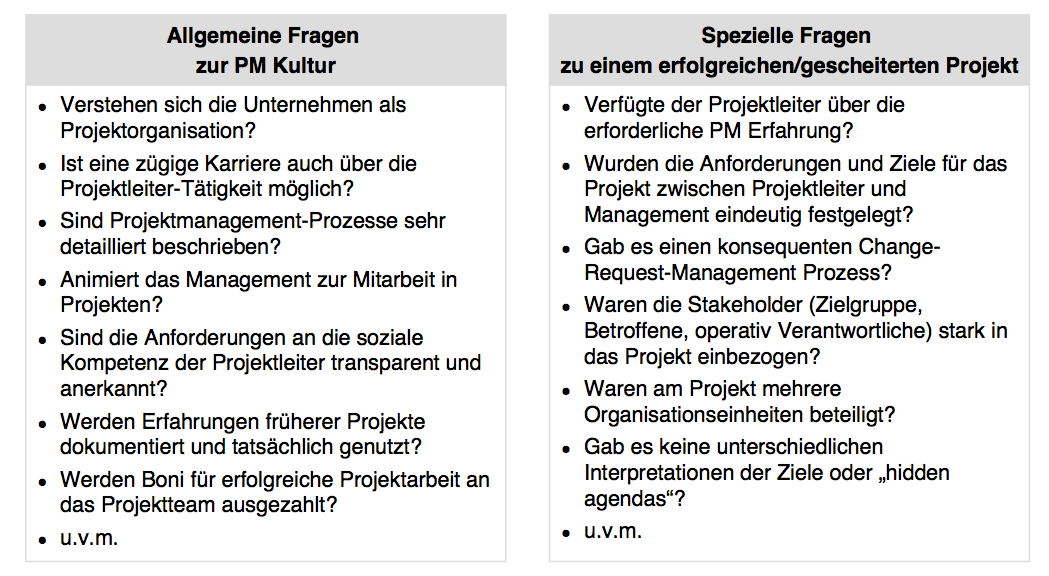
\includegraphics[width=0.9\textwidth]{img/fragen_gpm_studie}
		\caption{Fragen der GPM-Studie}
		\label{fragen_gpm_studie}	
	\end{center}
\end{figure}
\ 
\\
Für die vorliegende Ausarbeitung ist allerdings wesentlich interessanter, was die Gründe für Erfolg oder Misserfolg von einzelnen Projekten sind. Zu diesem Thema hat die GPM die teilnehmenden Unternehmen zu erfolgreichen und gescheiterten Projekten befragt. Für die Auswertung der Einzelprojekte wurde folgende Methodik angewandt\footnote{Vgl. \cite{GPM_Studie_2008, Seite 9}}: %TODO: footnote
\begin{itemize}
    \item{Fragen für erfolgreiche und gescheiterte Projekte sind identisch}
    \item{Für jede Frage wurde aus jeder Antwort ein Durchschnittswert ermittelt; jeweils für ''erfolgreiches Projekt'' und für ''gescheitertes Projekt''}
    \item{Durchschnittswert liegt zwischen 1 (''trifft überhaupt nicht zu'') und 5 (''Trifft voll und ganz zu'').}
    \item{Durchschnittswerte einer Frage wurden den beiden Projektkategorien (gescheitert, erfolgreich) gegenübergestellt}
    \item{Differenz soll Aufschluss über Faktoren für Projekterfolg liefern}
\end{itemize}
\
\\
Details zu den Ergebnissen finden sich in den Abschnitten \ref{ergebnis_pmk} (Projektmanagement-Kultur) und \ref{ergebnis_einzel} (Einzelprojekte).

\subsubsection{Teilnehmer}

Neben der Frage \textit{welche} Daten erhoben werden, muss auch geklärt werden, \texttt{wer} an der Studie teilgenommen hat. Dies waren 79 Unternehmen, überwiegend Organisationen mit mehr als 1000 Mitarbeitern und mit überwiegend Jahresumsätze von mehr als 1 Mrd. EUR (\textit{Vgl. siehe \cite{GPM_Studie_2008}, Seite 4}).\\
Es wurde versucht eine hohe Branchenvielfalt zu erreichen. Die Abbildung \ref{teilnehmer_gpm_studie} zeigt die prozentuale Teilnahme verschiedenster Branchen am Markt. Zu erwähnen sei noch, dass ein hoher Anteil von Unternehmen teilgenommen hat, die schon an früheren Studien der GPM oder PA-Group teilgenommen haben. 

\begin{figure}[H]
	\begin{center}
		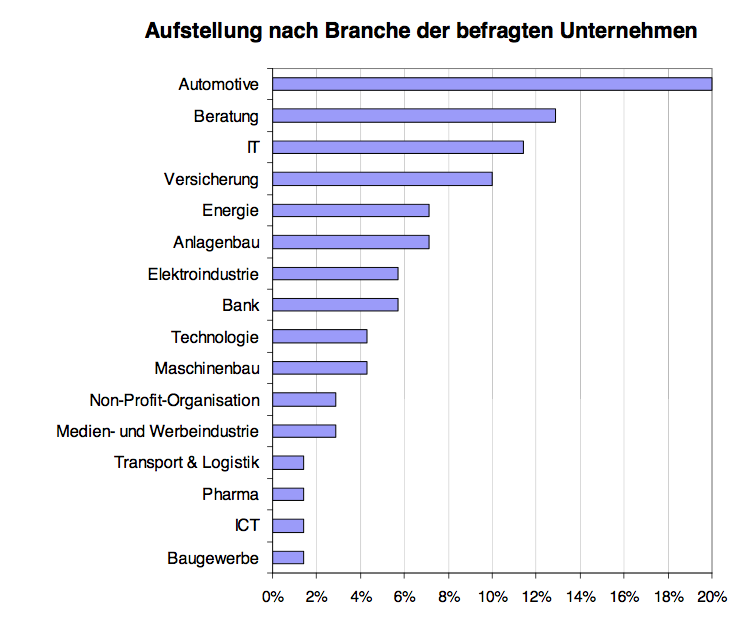
\includegraphics[width=0.9\textwidth]{img/teilnehmer_gpm_studie}
		\caption{Teilnehmer der GPM-Studie}
		\label{teilnehmer_gpm_studie}	
	\end{center}
\end{figure}

\subsubsection{Ergebnis der Projektmanagement-Kultur}
\label{ergebnis_pmk}
Das Ergebnis der Befragung der Projektmanagement-Kultur ist in Abbildung \ref{erfgebnis_gpm_studie_pmk} zu sehen. Fragen konnten nach einem Notensystem beantwortet werden, wobei 1 für ''Trifft gar nicht zu'' und 5 für ''Trifft voll und ganz zu'' einzusetzen waren. \\
Als \texttt{schwach} werden diejenigen Fragen bewertert, die weniger als 3,5 in ihrem Durchschnittswert erzielt haben. Hier herrscht Optimierungsbedarf. 

\begin{figure}[H]
	\begin{center}
		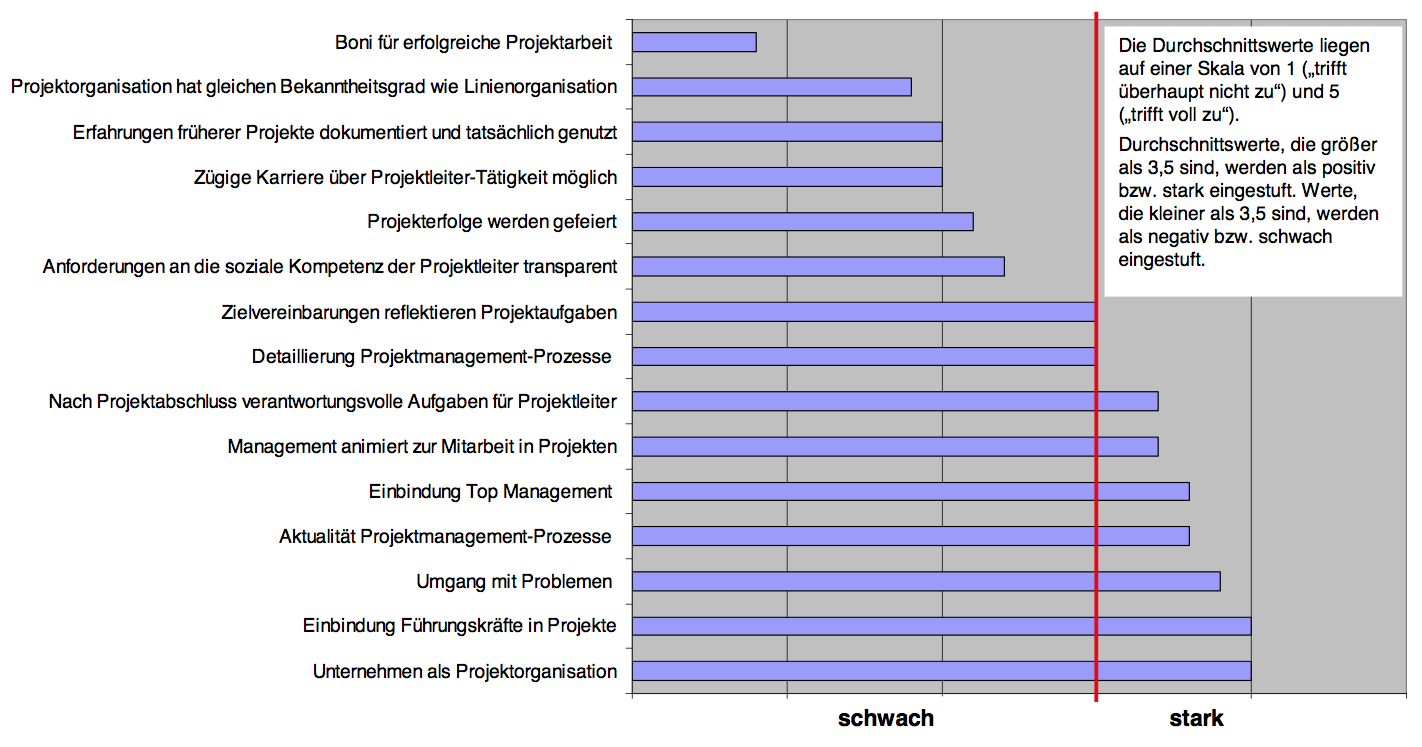
\includegraphics[width=1.0\textwidth]{img/ergebnis_gpm_studie_kultur}
		\caption{Ergebnis der GPM-Studie der Projektmanagement-Kultur}
		\label{erfgebnis_gpm_studie_pmk}	
	\end{center}
\end{figure}
\ \\
Wie in Abbildung \ref{erfgebnis_gpm_studie_pmk} zu sehen ist werden zu wenig Boni für erfolgreiche Projektarbeit angeboten und den Projektleitern geringe Karrierechancen eingeräumt. Es fehlt also überwiegend ein Anreizsystem, um sich den Aufgaben als Projektleiter zu stellen und die nötige Motivation für diese Tätigkeit.\\
\\ 
Projektorganisation gleicht der Linienorganisation. Es werden zu wenig Erfahrungen aus früheren Projekten dokumentiert und in anderen Projekten genutzt.

\subsubsection{Ergebnis Einzelprojekte}
\label{ergebnis_einzel}

Wie im Abschnitt \ref{erhobene_daten} beschrieben, galt es durch verschiedene Fragen an Projektbeteiligte von gescheiterten und erfolgreichen Projekten und Gegenüberstellungen dieser Fragen bestimmte Erfolgsfaktoren für Projekte zu ermitteln. Die Abbildung \ref{ergebnis_gpm_erfolgsfaktoren} zeigt die Top-10 der Gewichtungen der Antworten mit den größten Differenzen. Das rote Polygon zeigt die Gewichtung der gescheiterten Projekte und das blaue Polygon zeigt die Gewichtung der erfolgreichen Projekte. 

\begin{figure}[H]
	\begin{center}
		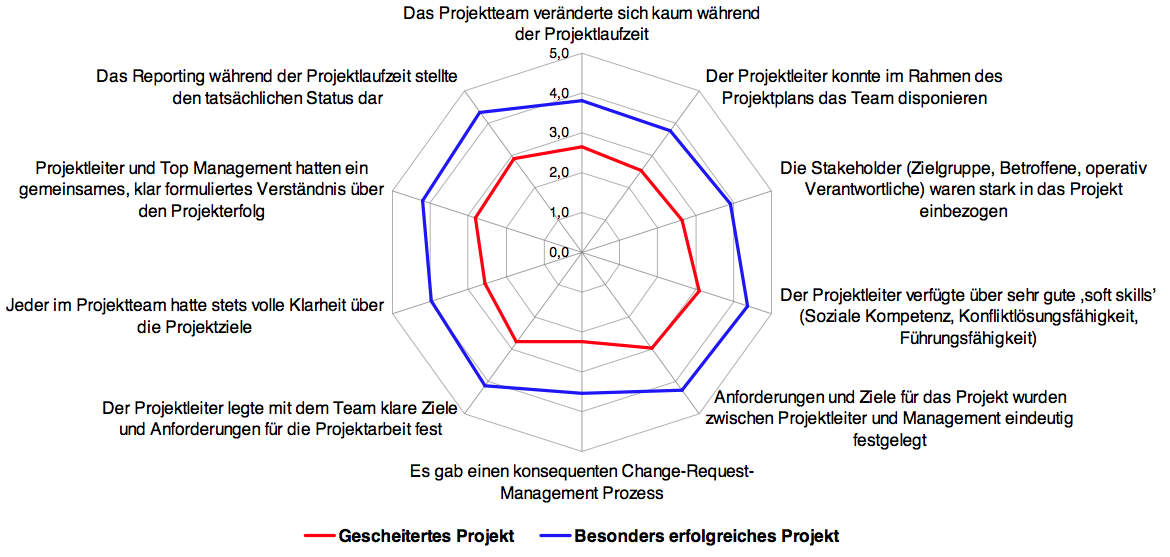
\includegraphics[width=1.1\textwidth]{img/ergebnis_erfolgsfaktoren}
		\caption{Die Erfolgsfaktoren in gescheiterten und erfolgreichen Projekten}
		\label{ergebnis_gpm_erfolgsfaktoren}	
	\end{center}
\end{figure}
\ \\
Die in Abbildung \ref{ergebnis_gpm_erfolgsfaktoren} zu sehenden Antworten wurden von der GPM in sechs Cluster gruppiert. Dort bestätigen sich die bisherigen Ergebnisse. Kommunikation, Zielvorgaben und Projektleiterposition sind die häufigsten Faktoren, die  den Erfolg eines Projekts beeinflussen. Die Abbildung \ref{ergebnis_gpm_gruppiert} zeigt die sechs Cluster nach der Gruppierung der Antworten. 

\begin{figure}[H]
	\begin{center}
		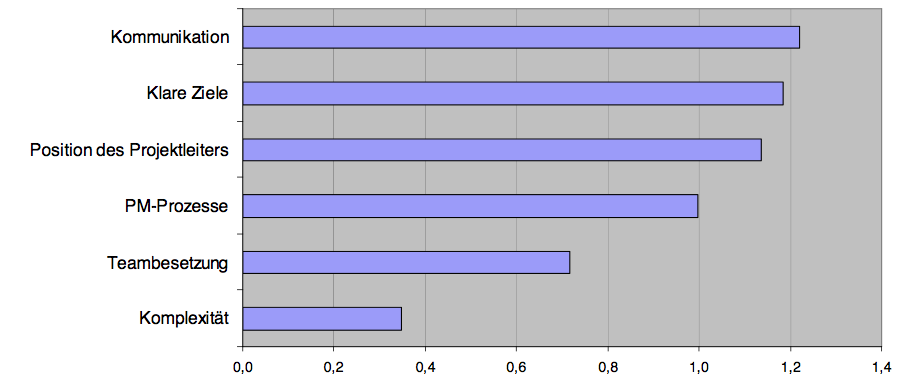
\includegraphics[width=0.9\textwidth]{img/ergebnis_gpm_gruppiert}
		\caption{Gruppierung der Ergebnisse}
		\label{ergebnis_gpm_gruppiert}	
	\end{center}
\end{figure}


\subsection{Vergleich und Auswertung}

Nach Auswertung der Fragen zur Projektmanagementkultur kam das Ergebnis zustande, dass Anreize fehlen, um sich als Projektleiter zu engagieren. \\
Das Ergebnis zur Befragung von Einzelprojekten gab Aufschluss das Kommunikation, Zielvorgaben und die Position des Projektleiters entscheidend seien. Es gibt dementsprechend wenig Anreize für Projektleiter sich in ihrer Position besonders zu engagieren, aber gleichzeitig ist der Projektleiter von besonders entscheidener Bedeutung im Projekt. Ebenfalls spielt die berufliche Position des Projektleiters eine Rolle.\\
Ein generelles Problem ist die Kommunikation, wobei andere Problembereiche auch zur Kommunikation zurückgeführt werden können, bzw. Kommunikation meist ein Teilproblem aller Probleme darstellt.\\
Weiterhin werden Projektziele als wichtiger Erfolgsfaktor genannt. Gerade bei den Antworten der Befragten bezüglich gescheiterter Projekte wurden Projektziele kritisiert  (siehe Abbildung \ref{ergebnis_gpm_erfolgsfaktoren}).\\
\\
Im Vergleich mit anderen Studien, wie zum Beispiel \cite{euregio__studie_erfolgsfaktoren}, fällt das Ergebnis ähnlich aus. Dort wurden 5700 Projekte in 44 Studien untersucht. Die Top-3-Erfolgsfaktoren sind hier: \textit{Kommunikation}, \textit{Zieldefinition}, \textit{Planung}. Ganz ähnlich zu den Ergebnissen der GPM-Studie.\\
\\
Eine weitere Studie der GPM\footnote{\cite{gpm_gesamt_07_09}} aus dem Jahre 2008/2009 zum Stand und Trend des Projektmanagements, welche sich mit den Forschungsgebieten im Projektmanagement beschäftigt, zeigt auf, dass die speziellen Teilgebiete \textit{Projektplanung}, \textit{Termin-}, \textit{Kosten-}, \textit{Change-} und \textit{Konfliktmanagement} nach Expertenaussagen ausreichend erforscht wurden (Vgl. siehe \cite{gpm_gesamt_07_09}, Seite 5). Hier bestätigen sich die Erfolgsfaktoren aus der GPM-Studie von 2008 Erfolg und Scheitern im Projektmanagement. Zum Beispiel sind Projektziele ein wichtiger Erfolgsfaktor, welche der Projektplanung zugeordnet werden können. Die Studien liegen dieser Ausarbeitung als Anhang bei. \\
\\
Insgesamt können aus der vorgestellten Studie und dem Vergleich mit weiteren Studienergebnissen die folgenden Erfolgsfaktoren abgeleitet werden:
\begin{itemize}
    \item{Kommunikation}
    \item{Projektziele}
    \item{Teambesetzung und Projektleiterposition}
    %\item{Ressourcenverteilung und PM-Prozesse}
\end{itemize}
Die aufgelisteten Erfolgsfaktoren sollen in den folgenden Abschnitten näher beleuchtet werden, sowie Probleme festgestellt, beschrieben und Führungstipps gegeben werden.

\pagebreak
\section{Kommunikationsprobleme}
\label{kommunikationsprobleme}

Aus der vorgestellten Studie (\cite{GPM_Studie_2008}, siehe Abschnitt \ref{projekte_scheitern}) geht hervor, dass Kommunikation am meisten zum Projekterfolg beiträgt. Es ist \textit{der} Erfolgsfaktor, da Probleme zu jeder Zeit und in jeder Phase ausftreten können und nur schwer zu beseitigende Spuren bei Projektbeteiligten hinterlassen können. Dieser Abschnitt widmet sich den Problemen der Kommunikation in Projekten.

\subsection{Sprachbarrieren und kulturelle Eigenheiten}
In global orientierten Projekten und Projekten mit internationaler Besetzung der Projektbeteiligten werden höchstwahrscheinlich Kommunikationschwierigkeiten auftreten. Zum einen können Probleme aufgrund von Sprachbarrieren entstehen und zum anderen können spezielle kulturelle Eigenheiten dazu beitragen, dass Schwierigkeiten auftreten. \\
\\
Ein Beispiel für Sprachbarrieren wären Dialekte, die es erschweren, trotz einer geeinigten Projektsprache, Projektbeteiligte akustisch zu verstehen. Schriftliche Kommunikation, zum Beispiel E-Mail, Foren, Wikis usw., ist oft nicht geeignet, wenn es darum geht Entscheidungen schnell zu treffen. Telefonkonferenzen oder persönliche Meetings schaffen zum einen Vertrauen in Projektbeteiligte und führen auch zur aktiven Entscheidungsfindung (alle Entscheidungsträger an einem Ort). Es kann an dieser Stelle jedoch zu dem Problem der Sprachbarrieren kommen. Nachfolgend ein Beispiel: \\
In einem Projekt mit internationalen Projektbeteiligten aus Russland, Deutschland, Indien und Japan soll eine Telefonkofnerenz zum aktuellen Stand eines Projekts gehalten werden. Als sprachliche Kommunikationsgrundlage soll Englisch verwendet werden. Das Problem liegt auf der Hand: Während der Telefonkonferenz unterliegen die russischen, indischen, japanischen und auch die deutschen Dialekte beim Englisch einigen Schwierigkeiten und die Kommunikation leidet. Bei längeren Meetings wird erneutes Nachfragen und das Wiederholen von Gedanken und Informationen frustrierend. Technische Störungen in Verbindungen tragen ebenfalls zu Behinderungen bei. Bestimmte Informationen sind nicht bei allen Projektbeteiligten angekommen und können beim Protokoll zu weiteren Schwierigkeiten führen. \\
Ein weiteres Problem, das bei einem persönlichen Meeting auftreten kann: Kulturelle Unterschiede. So könnte zum Beispiel die Verbeugungshaltungen in der japanischen Kultur bereits bei der Begrüßung zu Problemen führen. \\
\\
Wie in dem Artikel, \cite{nur_emails_sind_zu_wenig}, geschrieben, müssen vor allem Werkzeuge zur Kommunikation gewählt werden. Ein reiner E-Mail-Verkehr reicht nicht aus. Gerade bei Problemen, die durchaus auch Thema der Kommunikation sein dürfen und auch sollten, ist Reflexionsfährigkeit ein Muss. Auch darf es in einem Projekt nicht dazu führen, dass Projektbeteiligte die hierarchischen Abläufe scheuen. Die Kommunikationskultur sollte offen, ehrlich und glaubwürdig sein.

\subsection{Fachsprache}
Unterschiedliche Fachsprachen können oft ein großes Problem darstellen. In IT-Projekten sind typische Projektbeteiligte, die an der Umsetzung des Projekts beteiligt sind, Software-Entwickler, Programmierer und IT-Fachleute. Auf der anderen Seite gibt es oft BWL-Fachleute, die auch zu den Teams gehören und häufig leitende Rollen im Projekt inne haben. Je nach Hintergrund des jeweiligen Projektbeteiligten kann es zu Schwierigkeiten in der Kommunikation und dem Verständnis über Vereinbartes kommen. Dies liegt allzu oft an den unterschiedlichen Fachsprachen der Beteiligten. \\
\\
Als Beispiel soll folgendes, imaginäres Projektziel dienen:
Für einen Onlineshop sollte ein Betrugsabwehrsystem implementiert werden. Dazu wurde extern eine Schnittstelle eingekauft, die Daten über Neukunden auswertet und eine Empfehlung über Zahlarten zurückliefert. Bei der Implementierung entstanden Probleme mit der HTTP-Kommunikation und Kodierungsprobleme beim Empfang.\\
Zur Absprache setzten sich die betrauten Programmierer mit dem Implementierungsmanager der externen Zulieferer zusammen. Der Projektleiter wurde über den Fortschritt in Kenntnis gesetzt und verstand die Problematik der Kodierung der HTTP-Nachrichten nicht, da der Projektleiter wenig Kenntnisse über die technischen Abfolgen der Betrugsabwehr besaß. Die Folge waren interne Kommunikationschwierigkeiten die auch die Umsetzung erschwerten.\\ 
\\
Zur Lösung des Problems kann eine Kommunikationskultur etabliert werden. Auch die Schulung des Personals auf die jeweiligen Fachgebiete kann dazu betragen, dass Kommunikation im Projekt und das Verständnis für diese verbessert wird. 

%TODO: schreiben
\subsection{Zuviel, wenig und falsche Kommunikation}
Ein wesentlicher Faktor für Probleme in der Kommunikation ist deren Menge. Das Kommunizieren im Projekt ist wichtig und unabdingbar, allerdings kann ein Projekt auch der vermehrten Kommunikation unterliegen, in der das Gefühl entsteht, dass das Projekt keinen Fortschritt aufzuweisen hat, da zuviel kommuniziert wird und zu viele Ideen im Nachhinein in ein Projekt integriert (zumindest versucht) werden. Auf der anderen Seite kann das Gefühl für das Projekt verloren gehen, wenn zu wenig oder garnicht kommuniziert wird.\\ Auch sollte Kommunikation von unterschiedlichen Projektbeteiligten immer ehrlich und gründlich geschehen. Probleme nicht auszusprechen oder Informationen geheim zu halten sind echte Projektkiller und machen das Vertrauen in die eigene Person zunichte.\\

%\pagebreak
%\framebox{
%	\colorbox{red!20}{
%		\parbox{0.44\textwidth}{
%Dolore te feugait nulla facilisi nam liber tempor cum soluta nobis eleifend option. Amet consectetuer adipiscing elit sed diam nonummy nibh euismod tincidunt ut laoreet. In iis qui facit eorum; claritatem Investigationes demonstraverunt lectores legere me. In vulputate velit esse molestie consequat vel illum dolore. Wisi enim ad minim, veniam quis nostrud exerci. Facer possim assum typi non habent claritatem insitam est usus legentis lius quod.
%		}
%	}
%}
%\framebox{
%	\colorbox{green!20}{
%		\parbox{0.44\textwidth}{
%Dolore te feugait nulla facilisi nam liber tempor cum soluta nobis eleifend option. Amet consectetuer adipiscing elit sed diam nonummy nibh euismod tincidunt ut laoreet. In iis qui facit eorum; claritatem Investigationes demonstraverunt lectores legere me. In vulputate velit esse molestie consequat vel illum dolore. Wisi enim ad minim, veniam quis nostrud exerci. Facer possim assum typi non habent claritatem insitam est usus legentis lius quod.
%		}
%	}
%}

\pagebreak
\section{Projektziele}
%\begin{quote}
%\colorbox{blue!5}{\textbf{Fleiß für die falschen Ziele ist noch schädlicher als Faulheit für die richtigen.}}\footnote{Peter Bamm (1897 - 1975, dt. Arzt u. Schriftsteller)}
%\end{quote}
\ \\
Ein weiterer Faktor für den Projekterfolg ist nach den Studien aus dem Abschnitt \ref{projekte_scheitern} die Zieldefinitionen eines Projekts. Dieser Abschnitt beschäftigt sich mit Problemen in der Zielsetzung eines Projekts. 

\subsection{Zielfindung und -darstellung}

Die Zielfindung eines Projekts kann im wesentlichen auf zwei Arten geschehen:
\begin{itemize}
    \item{intuitives Brainstorming\footnote{Es werden mehr oder weniger Zielvorstellungen intuitiv gesammelt.}}
    \item{systematischen Ableiten\footnote{Aus einem Oberziel wird versucht systematisch weitere Ziele abzuleiten.}}
\end{itemize}
\ \\
Welche Art gewählt wird, hängt von den Beteiligten, dessen Erfahrungswerte und der Art des Projekts ab. Es sei auch gesagt, dass die Präzisierung von Zielen gerade in der Anfangsphase eines Projekts höchstwahrscheinlich mehrmals vorgenommen wird, da die Details über die Ziele erst mit dem Beginn der Realisierung deutlich werden. \\
Hier könnte ein erstes Problem vorhanden sein: Wer ist beteiligt an der Zielfindung eines Projekts?\\ 
An der Zieldefinitionsphase sollten auf jeden Fall das Projektmanagement, der Projektleiter, Projektmitarbeiter und, sehr wichtig, der Auftraggeber beteiligt sein. Im Zweifelsfall sollten alle Projektbeteiligten am Zielfindungspozess mitarbeiten. Nur so kann eine engere Zusammenarbeit gewährleistet werden.\\
\\
Ein weiteres Problem, das sich aus der Zielfindung ergibt, ist die Zieldarstellung. Sind die Projektziele verständlich visualisiert (Kann jeder Projektbeteiligte es verstehen oder kann es unterschiedlich gedeutet werden)? Welche Prioritäten liegen auf den einzelnen Projektzielen? \\
\\
Zur Lösung der Probleme der Zielfindung und -darstellung können verschiedene Ansätze verwendet werden:
\begin{itemize}
    \item{Kick-Off-Meetings}
    
    \item{Workshops}
    
    \item{UML, Layouts, Wireframes, Mock-ups}
    
    \item{Problemlösungszyklusmethode}
    
\end{itemize}
\ \\
Bei \textit{Kick-Off-Meetings}, auch \texttt{Auftakt-Sitzung} genannt, wird versucht ein neu zu beginnendes Projekt einen \textit{optimalen} Start zu verschaffen. Es prägt in vielerlei Hinsicht die Erwartungshaltungen der Projektbeteiligten an das Projekt. Das erste mal treffen alle Projektbeteiligten aufeinander und es werden, neben Zwischenmenschnlichen Signalen, auch fachliche Inhalte geklärt. Es bedarf guter Vorbereitung und sollte die Rollenverteilung im Projekt, sowie den Nutzen des Projektergebnisses klären. \\
\\
\textit{Workshops} sind eine gute Möglichkeit alle Projektbeteiligten auf fachliche Details des Projekts einzustimmen und um die ''Mannschaft auf Kurs'' zu bringen. Wie in allen Workshops sollte dies moderiert werden, um alle Punkte der Workshop-Agenda abzuarbeiten und es sollte, je nach größe der zu klärenden Fragen, terminierbar sein. Bei großen Projekten kann ein Workshop mehrere Tage beinhalten. Allerdings sollte der Workshop nicht unterbrochen werden, damit alle Projektbeteiligten fokussiert werden können. \\
\\
Zur Zieldarstellung und um für alle Prjektbeteiligten ein Gesamtbild der Ziele zu schaffen bietet es sich immer an ein vorläufiges Ergebnis zu erarbeiten. Dies kann beispielsweise ein \textit{Wireframe} sein. Es dient der schematischen Darstellung des Produkts. Bei vielen Projektmitarbeitern kann auch die Verwendung von \textit{UML}-Diagrammen zur besseren Zieldarstellung verhelfen. Zum Beispiel kann mittels UML der Kommunikationsablauf zwischen Clients und dem zentralen Serverdienst aufgezeigt werden. Zur Darstellung des Software-Frontends können \textit{Layouts} verwendet werden. Damit hat meist ein externer Auftraggeber einen guten Überblick auf das Projektziel und damit auf das Produkt. Gerade in Software-Projekten hat sich die Verwendung von sog. \textit{Mock-Ups} etabliert. \\
\\
Bei der Verwendung der \textit{Problemlösungszyklusmethode}, siehe Abbildung \ref{probsolcycle} (entnommen aus Präsentation von \cite{slishare_einf_pm}), werden systematisch und schrittweise nach einem Leitfaden Ziele gefunden und zur Zieldefinition hinzugefügt. Es bietet sich zum Beispiel an, wenn der Auftraggeber wenig Vorstellung über das zu schaffende Produkt hat oder wenn keine detaillierten Ziele auf Anhieb gefunden werden können. 

% TODO: Grafik überarbeiten
\begin{figure}[H]
	\begin{center}
		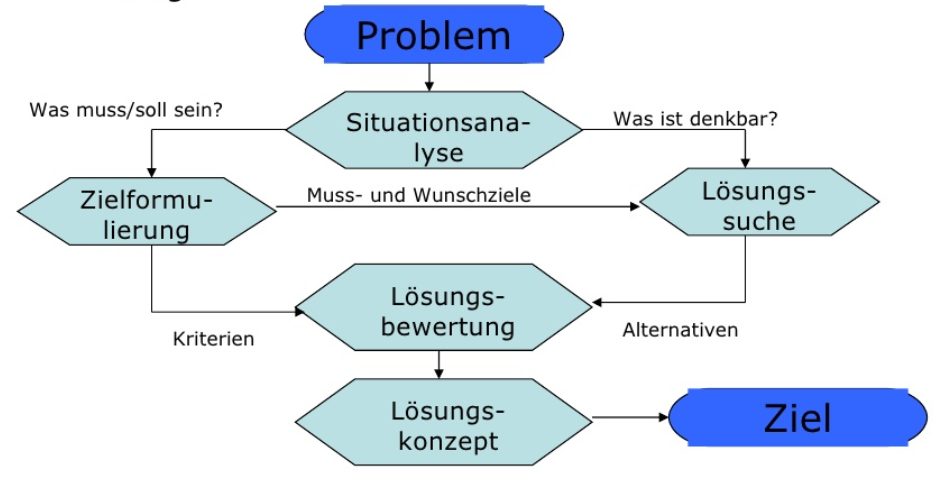
\includegraphics[width=1.0\textwidth]{img/problemloesungszyklus}
		\caption{Zielfindungsmethode: Problemlösungszyklus}
		\label{probsolcycle}	
	\end{center}
\end{figure}

\subsection{Zielformulierung}
Hauptursache für Probleme in einem Projekt sind oft schlecht formulierten Projektziele. Unklare Projektziele führen zu:
\begin{itemize}
    \item{erhöhten Projektkosten}
    \item{Verschwendung von Projektressourcen}
    \item{meist zu zuviel Kommunikation}
    \item{Nicht-Einhaltung des Zeitplans}
\end{itemize}
\ \\
Nachfolgend das Beispiel: \\ 
\\
\texttt{Die Request-Response-Zeiten sollen verbessert werden.}\\
\\
Das obige Beispiel beinhaltet mehrere Probleme. Zum einen geht aus der Formulierung nicht hervor bis wann die Request-Response-Zeiten verbessert werden sollen. Es ist auch nicht bekannt was eine Verbesserung darstellt. Auch kann aus dem Kontext der Zielformulierung der Umfang der Aufgabe nicht abgeleitet werden. Die Formulierung könnte weiterhin aktiv geschrieben werden. Es ist unklar wer im Projekt die Aufgabe übernimmt. Soll es das Kernentwicklerteam übernehmen oder wird es von externen Mitgliedern übernommen?\\
\\
Gute und richtige Zielformulierungen lassen sich wie folgt definieren: 
\begin{itemize}
    \item{Zielformulierungen sollten S.M.A.R.T: Spezifisch, Messbar, Akzpetiert, Realistisch und Terminierbar sein}
    \item{Es sollte positiv und aktiv formuliert werden\footnote{aktive- und positve Formulierung: Wort wie \textit{verringern}, \textit{nicht} usw. vermeiden. und Aktivität klären (interne Bearbeitung, externe Zuliferer)}}
    \item{Projektziele sollten in kleinen, abgetrennten - dafür genauen - Zielen formuliert sein}
    \item{Definition von Meilensteinen}
\end{itemize}
\ \\
Damit lassen sich verschiedene Punkte des Beispiels umformulieren, bzw. erweitern, damit die Zielformulierung verbessert wird:\\
\\
\texttt{Die Request-Response-Zeiten sollen vom internen Entwicklerteam des\\
Projekts um 10 \% bis 31.12.2013 verbessert werden.} \\
\\
Das überarbeitete Beispiel behebt die Probleme mit der Zieldarstellung in dem es das Ziel spezifiziert (Was verbessert werden soll), terminiert und die Zuständigkeit im Projekt klärt.


\subsection{WISCY-Syndrom}
\label{wiscy_syndrom}
Ein Problem, mit dem ein Projektmanagement konfrontiert werden kann, ist das in den USA benannte \texttt{Why isn`t Sam coding yet?}-Syndrom - frei übersetzt: Warum ist der Bursche noch nicht am programmieren? (Vgl. \cite{proj_zum_erfolg_fuehren}, Kaptiel 7 Seite 85) \\
Zu oft möchte man als Team schnell mit der Realisierung beginnen oder der Projektleiter will schnell erste Resultate erhalten. Sehr oft wird die Zieldefinitionsphase dabei voreilig beendet. Das Ergebnis sind meist unklare Ziele und schlechte Zielformulierungen, die im späteren Projektverlauf dann teuer korrigiert werden müssen.\\
\\
Wie kann diesem Syndrom Abhilfe geschaffen werden? Hier kann die Führungsetage die Zieldefinitionen kontrollieren und nach der Eindeutigkeit prüfen lassen. Nur wenn gewissenhaft die Projektziele klar - und damit für jeden Projektbeteiligten verständlich - sind kann mit der Umsetzung begonnen werden.

\pagebreak
\section{Teambesetzung und Projektleiter}
Bei einem Projekt sind immer verschiedene Beteiligte aus unterschiedlichen Positionen eines Unternehmens vertreten. In manchen Projekten auch aus unterschiedlichen Unternehmen. Von besonderer Wichtigkeit ist hier der Projektleiter, bzw. dessen Position im Unternehmen. Auch ist es wichtig wie die einzelnen Projektbeteiligten und Teammitglieder zusammen arbeiten. Konflikte können überall unter Teams entstehen, weswegen es wichtig ist, dass harmonierende Personen ein Team bilden. 

\subsection{Teambesetzung}
\label{teambesetz}
Falsche Teambesetzung kann schnell zum Stagnieren eines Projekts führen. Hier sind allzu oft fehlendes Vertrauen, Interessenskonflikte und seltener Antipathien als Gründe zu nennen. Die Interessenskonflikte bei großen Projekten, in den sich sogar mehrere Unternehmen die Arbeit teilen, können große Schwierigkeiten verursachen. Weiterhin kann es zu Polarisierung in einem Projektteam kommen.\\
\\
Wie im Abschnitt \ref{proj_beteiligte} beschrieben, können Projektbeteiligte in drei Gruppen unterschieden werden. Gerade zwischen diesen Gruppen und weiteren Unterscheidungen zwischen internen Kunden, also den Projektmitarbeitern, und Zulieferern kann es schnell zu Interessenskonflikten kommen und Rivalitäten enstehen. Auch sind in internationalen Projekten kulturelle Unterschiede oft ausschlaggebend für Probleme im Team und bei der Projektumsetzung.\\
\\
Bei konkurrierenden Teams und verschiedenen Unternehmen, die zur Zusammenarbeit im Rahmen des Projekts gezwungen werden, kommt es oft zu fehlenden Vertrauen in die Arbeit des jeweils anderen Teams. Bei Problemen wird die Frage nach der Ursache bei anderen Teammitgliedern oder Teams gesucht. \\
\\
Ein Beispiel bietet der Artikel \cite{deu_franz_pm}, in dem interkulturelle Projektarbeit analysiert wird. Es sind die unterschiedlichen Vorstellungen von Prozessabläufen und von der Zusammenarbeit, die die Produktivität und den Projektforschritt beeinträchtigen können. Auch ensteht beim interkulturellen Projektmanagement oft eine bestimmte Kulturdominanz\footnote{Kulturdominanz: Mehrere Leitende Personen \textit{einer} Kultur nutzen ihre eigenen Wertvorstellungen}.\\
Der Artikel gibt auch einen Lösungsvorschlag für die Schaffung einer \textit{interkulturellen Balance}. Es sollen Regeln für das Projekt geschaffen werden. Zum Beispiel die Projektsprache (meist Englisch in internationalen Projekten), aber auch Anpassungen an eigene Arbeitsstile. Es kann damit eine \textit{Interkultur}\footnote{Interkultur: Schaffung einer neuen "Kultur" durch das Zusammenwirken zweier oder mehrerer Kulturen in gemeinsamer Arbeit.} entstehen.

\subsection{Projektleiterposition}

Neben der Auswahl eines geeigneten Projektleiters\footnote{Vgl. siehe \cite{proj_zum_erfolg_fuehren}, Kapitel 6 Seite 67 ff.} kann die Position des Projektleiters im Unternehmen zu Problemen führen.\\ 
\\
Nachfolgend sei das folgende Beispiel gegeben:\\
In einem Projekt wurde ein Sachbearbeiter für ein mittleres Projekt mit dem Ziel ein neues Dienstleistungssegment zu analysieren eingesetzt. Dazu sollte prototypisch eine webbasierte Dienstleistungssoftware entwickelt werden.\\
Als junger Mitarbeiter im Unternehmen trat vor allem das Problem auf, dass unterschiedliche Abteilungen im Projekt involviert werden sollten. Beispielsweise wurde bei der Frage des Hostings der Projektleiter von unterschiedlichen Abteilungen befragt. Dies führte zum einen zur Überkommunikation, die eigentlich nicht notwendig war (Siehe Abschnitt\ref{kommunikationsprobleme}) und zum anderen zur Überforderung des Projektleiters. Nach mehreren Wochen des "Kompetenzgerangels" gab der Projektleiter seinen Posten freiwillig auf.\\
Ein anderes Beispiel: der Projektleiter besitzt eine führende Rolle im Unternehmen. Dies fördert zwar im besten Falle das jeweilige eigene Projekt, allerdings kann es passieren, dass andere Projekte im Unternehmen vernachlässigt werden. Es könnte sein, dass Entscheidungen oder Projektstarts zu schnell verabschiedet werden (siehe Abschnitt \ref{wiscy_syndrom}).\\
\\
Für den Projektleiter im ersten Beispiel existierte kaum Motivation den Posten weiter zu führen, auch wenn dies unter Umständen nicht das nötige Vertrauen für weitere Projektleiterarbeit mit sich bringt.\\
\\
Der Projektleiter sollte ergo neben der Eignung, den Aufgaben auch definierte Befugnisse besitzen.

%\pagebreak
%\section{Ressourcenverteilung und PM-Prozesse}

\pagebreak

\section{Fazit}
Die geschilderten Probleme in Projekten und dem Projektmanagement sind, trotz der weitreichenden Studien von \cite{euregio__studie_erfolgsfaktoren}, \cite{gpm_gesamt_07_09} oder \cite{GPM_Studie_2008}, immer wieder anzutreffen. Auch die Forschung auf den Gebieten sind meist ausreichend vorhanden.\\ 
\\
Kommunikation ist der Flaschenhals eines jeden Projekts, ist Teil jedes anderen Problems und trägt zu jedem Erfolgsfaktor bei. Wie der Satz heißt: Man kann nicht nicht kommunizieren. Keine Handlung ist ebenfalls eine Form der Kommunikation. Wie schafft man also im Unternehmen und im Projekt eine gute Kommunikation? Es sollte für das Unternehmen eine Kommunikationskultur geschaffen werden, die sich durch jedes Projekt zieht und durch das gesamte Unternehmen. Mit Hilfe von Werkzeugen, seien es nun Software oder Methoden zur Kommunikation, kann ein kohärenter Kanal geschaffen werden, mit dem sich jeder Projektbeteiligte auskennt und diesen nutzen kann.\\
\\
Probleme entstehen oft aus fehlenden Erfahrungswerten und der geringen Wiederverwendung von Erfahrung aus vergangenen Projekten. Fehler werden wiederholt. Ich vertrete auch die Meinung, dass schlecht definierte Projektziele die größte Ursache für gescheiterte Projekte sind. Im Nachhinein wird fast immer die Umsetzung des Projekts kritisiert. Was ist aber, wenn die Umsetzung garnicht das Problem war, sondern das Projekt von vorn herein zum Scheitern verurteilt war, da die Ziele schlichtweg nicht vernünftig aufgestellt worden sind?\\
\\
Im Abschnitt \ref{teambesetz} wurde das Thema der interkulturellen Balance beschrieben. Meiner Meinung nach ist dieses Problem in Software-Entwicklungsprojekten nur bedingt existent. Software-Entwickler haben meist ihren eigenen Arbeitsstil und ihre eigenen Methoden zur Synchronisation. Viel eher existiert das Problem der unterschiedlichen Fachsprachen, führt so zu Verständnisproblemen und zu Vetrauenseinbußen.\\
\\
Auch kann ich fehlendes Vertrauen in Projektbeteiligte als Gründe für Probleme im gesamten Projektverlauf nennen. Interessenskonflikte zwischen rivalisierenden Unternehmen in einem Projekt habe ich bereits selber kennen gelernt.\\

\pagebreak
\thispagestyle{empty}
\addcontentsline{toc}{section}{Literaturverzeichnis} % Eintrag ins Inhaltsverzeichnis
\bibliography{bib/bibliography}
\pagebreak
\appendix
\part{Anhänge}
\thispagestyle{empty}
\section*{Checkliste}
\begin{checklist} 
\item Wurden geeignete Kommunikationskanäle für das Projekt ausgewählt? 
\item Kommunikation findet in dafür vorgesehenen Kanälen statt?
\item Wird für Absprachen die (falls vorhanden) vorgesehene Projektsprache verwendet?
\item Existiert eine Kulturdominanz und kann diese ausbalanciert werden?
\item Haben alle Projektbeteiligten einen identischen Wissensstand für die Zieldarstellung?
\item Die Projektziele wurden S.M.A.R.T definiert?
\item Die Projektziele sind aktiv formuliert?
\item Die Projektziele sind positiv formuliert?
\item Finden Meetings häufig genug statt? Oder finden zu viele Meetings statt?
\item Wer sind die Ansprechpartner im Projekt? 
\item Existiert eine klare Rollenverteilung?
\item Wurde ein Konfliktmanagement eingerichtet?
\item Wurde ein Krisenmanagement eingerichtet?
\item Harmonisiert das Projektteam? 
\item Hat der Projektleiter ausreichend Befugnisse um seine Aufgabe zu erledigen?
\item Wurden Vertreter für die jeweilige Position gewählt?
\end{checklist} 

\pagebreak
\thispagestyle{empty}
\section*{CD zur Hausarbeit}
Auf der beiliegenden CD befindet sich die vorliegende Hausarbeit inklusive aller Anhänge.
% TODO: Anhänge hinzufügen
%
\includepdf[pages=-]{attachements/articles/interkulturelle_zusammenarbeit.pdf}
%
\includepdf[pages=-]{attachements/articles/nur_email_ist_zu_wenig.pdf}
%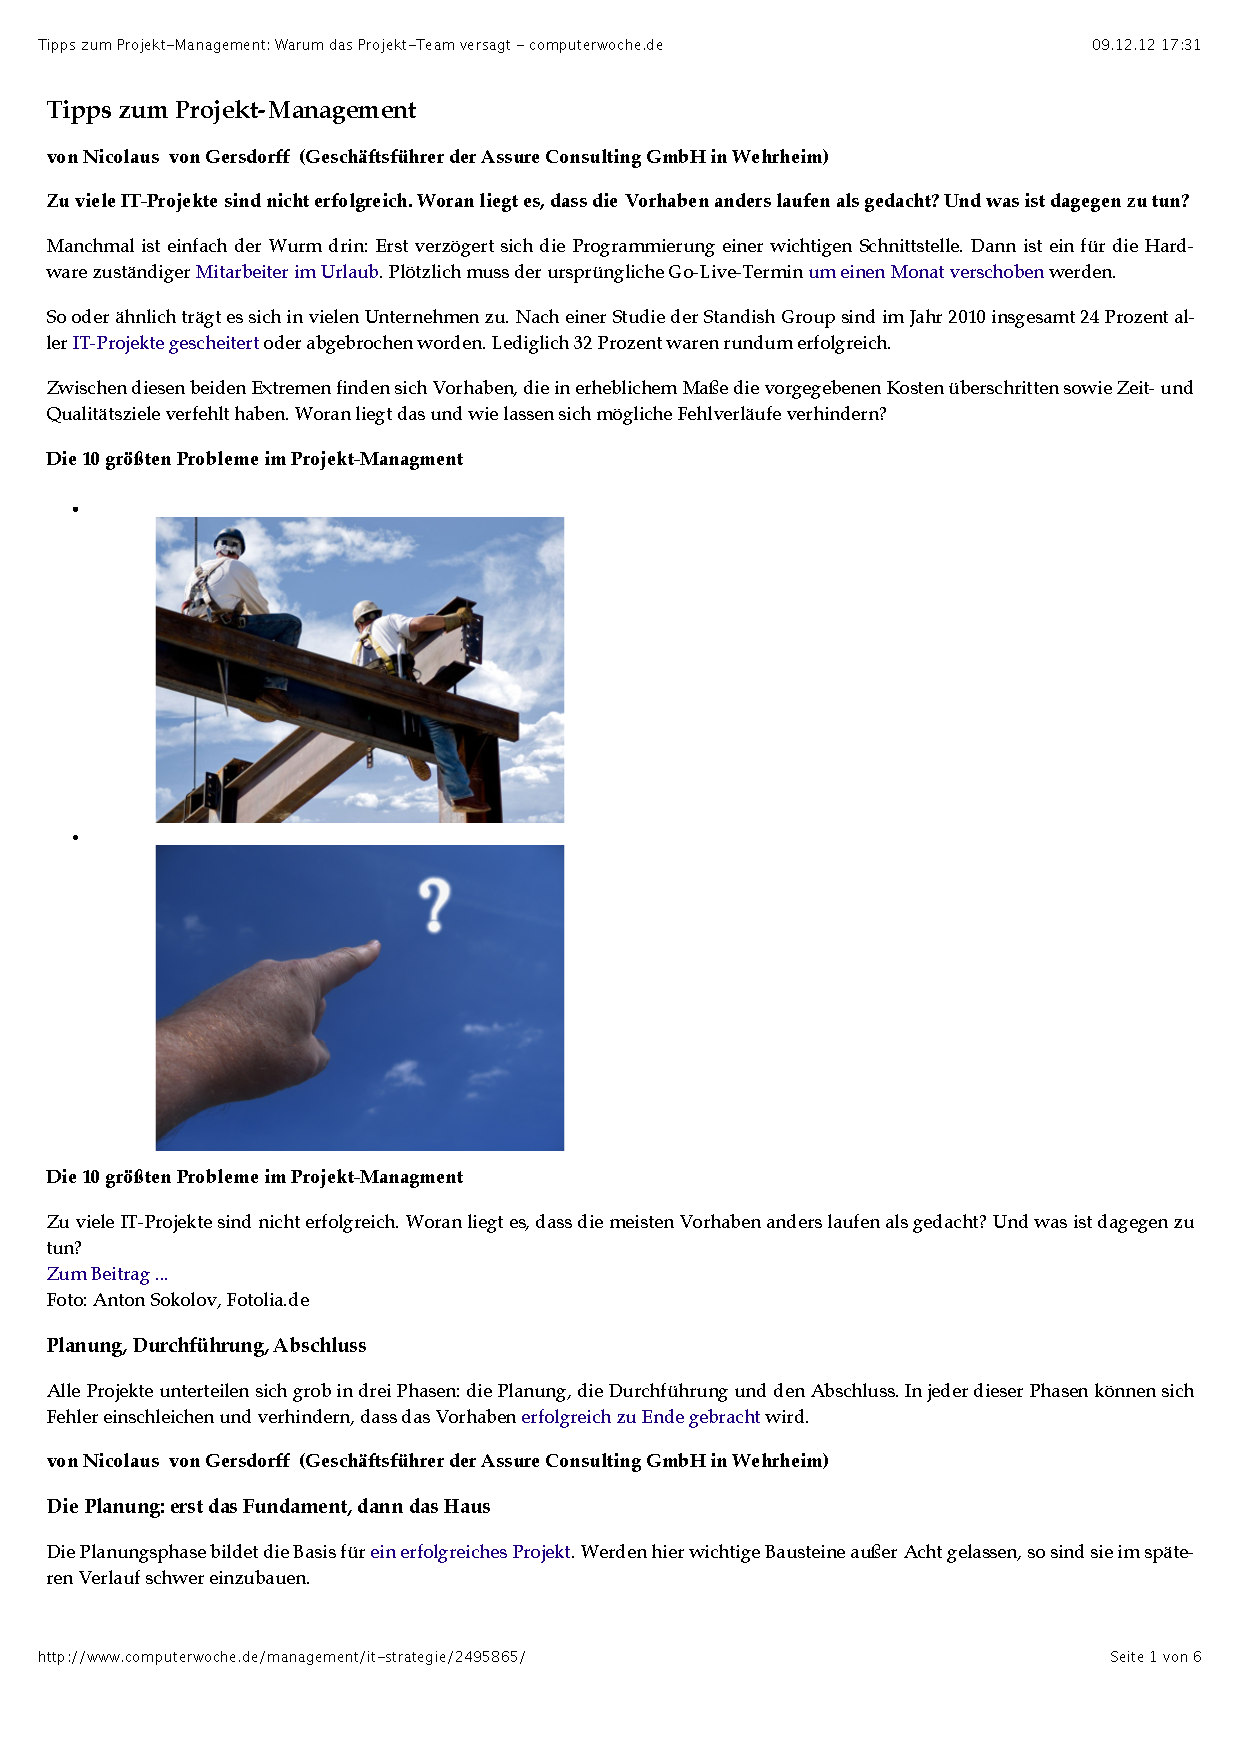
\includepdf[pages=-]{attachements/articles/tipps_zum_projekt.pdf}
%
\includepdf[pages=-]{attachements/studies/Ergebnisse_Erfolg_und_Scheitern-Studie_2008.pdf}
%\includepdf[pages=-]{attachements/studies/Gesamt-Studie-GPM-Juli_2009.pdf}
\end{document}
